\chapter{Confidential Guardian: Prohibiting the Abuse of Model Abstention}

\section{Additional Background on IT-MACs} \label{app:itmac}

\begin{contriback}
    This section was written by Olive Franzese.
\end{contriback}

Fix a field $\mathbb{F}_p$ over a prime number $p \in \mathbb{N}$, and an extension field $\mathbb{F}_{p^r} \supseteq \mathbb{F}_p$ for some $r \in \mathbb{N}$. We use the notation $\comm{x}$ to indicate that (i) $\prover$ is in possession of a value $x \in \mathbb{F}_p$, and a uniformly chosen tag $\mathbf{M}_x \in \mathbb{F}_{p^r}$ and (ii) $\verifier$ is in possession of uniformly chosen value-specific key $\mathbf{K}_x \in \mathbb{F}_{p^r}$ and a global key (which is the same for multiple authenticated values) $\Delta \in \mathbb{F}_{p^r}$. These values have the following algebraic relationship
\begin{align*}
\mathbf{M}_x = \mathbf{K}_x + \Delta \cdot x \in \mathbb{F}_{p^r}
\end{align*}
where $x$ is represented in $\mathbb{F}_{p^r}$ in the natural way. $\prover$ can \texttt{Reveal} an authenticated value by sending $x$ and $\mathbf{M}_x$ to $\verifier$, who then checks if the relationship holds. If it does not, then $\verifier$ knows that $\prover$ has modified $x$. $\prover$ and $\verifier$ can agree to modify an authenticated value while preserving the algebraic relationship and confidentiality over their respective values by exploiting linear homomorphism over IT-MACs, or by performing an interactive protocol to perform other arithmetic operations~\cite{damgaard2012itmac,nielsen2012itmac}. This idea is the basis of the ZKP protocol in~\cite{weng2021wolverine}. $\prover$ and $\verifier$ authenticate wire values which encode inputs to the circuit, and then compute secure transformations of the authenticated values in accordance with the operations required by the circuit (see~\cite{weng2021wolverine} for further details). By a standard completeness result in computability theory~\cite{sipser1996introduction}, composing secure additions and multiplications over authenticated values enables execution of any boolean predicate within a zero-knowledge proof. 


\section{Proof of Feasibility of Inducing Dishonest Uncertainty}
\label{app:region-manip-proof}

\begin{contriback}
This section was written by Olive Franzese.
\end{contriback}

We restate Lemma~\ref{lemma:region-manip} here, and provide a full constructive proof.

\begin{lemma} \label{restated-lemma:region-manip}
    Fix an arbitrary dataset $\mathcal{D}=\{(x_i, y_i)\}^{N}_{i=1}$ taken from feature space $\mathbb{R}^D$ and logits over a label space $\mathbb{R}^{C}$, and a set of feed-forward neural network model parameters $\theta$ encoding a classifier $f_{\theta}: \mathbb{R}^D \to \mathbb{R}^C$. Fix a set of indices $I$ such that for all $i \in I$, $i \in [1, C]$. For each index in $I$, fix bounds $a_i, b_i \in \mathbb{R}$ with $a_i < b_i$. Call $S$ the set of values $\mathbf{x} \in \mathbb{R}^D$ such that $a_i < x_i < b_i \quad \forall i \in I$. Then we can construct an altered feed-forward neural network $M'$ encoding $f'_{\theta}: \mathbb{R}^D \to \mathbb{R}^C$ which has the property $f'_{\theta}(x) = f_{\theta}(x) \quad \forall x \notin S$, and $f'_\theta(x)=f_\theta(x) + c \quad \forall x \in S$ where $c \in \mathbb{R}^C$ is an arbitrarily chosen non-negative constant vector.
\end{lemma} 

\begin{proof}
We design a collection of algorithms for constructing neurons which, when used to augment any feed-forward neural network $M$, specifically perturb the output logits of data points from an adversarially chosen region. 

We will use the notation $e_k$ to represent the $k^{th}$ unit basis vector (i.e. $e_k = (0, 0, ..., 0, 1, 0, ..., 0)$ where the $1$ is at the $k^{th}$ position). We will also name neurons, e.g. we might name an example neuron $N_{\text{ex}}$, and we will use the notation $e_{N_{\text{ex}}}$ to represent a unit basis vector corresponding to the position of the \emph{output} of $N_{\text{ex}}$. 

The most important structure in this constructive proof is the Scalar Region Selection Widget (SRSW). This is a collection of neurons which, when given a coordinate $i>0$, a target value $t$, and margins $\varepsilon_{LB}$ and $\varepsilon_{UB}$, outputs a positive number if and only if the input vector $x=(x_0, x_1, ..., x_i, ..., x_n)$ has $t - \varepsilon_{LB} < x_i < t + \varepsilon_{UB}$ and 0 otherwise. Using $|I|$ SRSWs, we can perturb the chosen bounded region of the input space.

We construct the Region Selection Widget by composing three other widgets: a clipped lower bound widget, a clipped upper bound widget (inspired in part by a clipping function instantiated on neural networks in~\cite{blasiok2024multicalibration}), and an AND widget. We describe them each below.

\textbf{Clipped Lower Bound Widget.} To construct a CLBW we design neurons to enact the function:
\begin{align*}
    f_{CLBW}(x, t)=\relu \left( \relu(\relu(x_i)-(t-\varepsilon_{LB})) - \relu(\relu(x_i-\varepsilon_{CLIP})-(t-\varepsilon_{LB}))) \right)
\end{align*}

The outputs of $f_{CLBW}$ are:
\[ \begin{cases} 
      0 & x_i \leq t - \varepsilon_{LB} \\
      y \in (0, \varepsilon_{CLIP}) & t-\varepsilon_{LB}<x_i<t-\varepsilon_{LB}+\varepsilon_{CLIP} \\
      \varepsilon_{CLIP} & t-\varepsilon_{LB}+\varepsilon_{CLIP} \leq x_i
   \end{cases}
\]

Given any $i, t, \varepsilon_{CLIP}$ and $\varepsilon_{LB}$ as input, the following series of neurons will compute $f_{CLBW}$: 
\begin{itemize}
    \item a neuron $N_1$ in the first hidden layer with weights $e_i$ and bias term 0
    \item a neuron $N_2$ in the second hidden layer with weights $e_{N_1}$ and bias term $-(t-\varepsilon_{LB})$
    \item a neuron $N_3$ in the first hidden layer with weights $e_i$ and bias term $-\varepsilon_{CLIP}$
    \item a neuron $N_4$ in the second hidden layer with weights $e_{N_3}$ and bias term $-(t - \varepsilon_{LB})$
    \item a neuron $N_5$ in the third hidden layer with weights $e_{N_2} - e_{N_4}$ and bias term $0$.
\end{itemize}

\textbf{Clipped Upper Bound Widget.} To construct this widget we design neurons to enact the function:
\begin{align*}
    f_{CUBW}(x, t) = \relu \left( \relu(-\relu(x_i)+(t+\varepsilon_{UB})) - \relu(-\relu(x_i + \varepsilon_{CLIP}) + (t + \varepsilon_{UB})) \right)
\end{align*}


Unlike the CLBW, here we must take as an assumption that $t$ is non-negative to achieve the desired functionality (this can be observed by inspecting $f_{CUBW}$). This assumption has no functional impact, as for any desired $t<0$, we can construct $t'=t+a$ such that $t+a>0$, and adjust input points by running them through a neuron with weights $e_i$ and bias term $a$, to achieve the same functionality as if we selected with threshold $t$. Keeping this in mind, we simply assume WLOG that $t$ is non-negative for the remainder of the proof. The outputs of $f_{CUBW}$ are then as follows:
\[ \begin{cases} 
      0 & x_i \geq t + \varepsilon_{UB} \\
      y \in (0, \varepsilon_{CLIP}) & t+\varepsilon_{UB}-\varepsilon_{CLIP} >x_i >t+\varepsilon_{UB} \\
      \varepsilon_{CLIP} & t+\varepsilon_{UB}-\varepsilon_{CLIP} \geq x_i \geq 0 
   \end{cases}
\]

Given any $i,t, \varepsilon_{CLIP},$ and $\varepsilon_{UB}$ as input, the following series of neurons will compute $f_{CUBW}:$
\begin{itemize}
    \item a neuron $N_6$ in the first hidden layer with weights $e_i$ and bias term $0$
    \item a neuron $N_7$ in the second hidden layer with weights $-e_{N_6}$ and bias term $(t + \varepsilon_{UB})$
    \item a neuron $N_8$ in the first hidden layer with weights $e_{i}$ and bias term $\varepsilon_{CLIP}$
    \item a neuron $N_9$ in the second hidden layer with weights $-e_{N_8}$ and bias term $(t + \varepsilon_{UB})$
    \item a neuron $N_{10}$ in the third hidden layer with weights $e_{N_7} - e_{N_9}$ and bias term $0$.
\end{itemize}

\textbf{Soft AND Widget.} We design neurons to enact the function:
\begin{align*}
    f_{AND}(o_1, o_2) = \relu(o_1 + o_2 - (2\varepsilon_{CLIP} - \varepsilon_{AND}))
\end{align*}
where $o_1$ and $o_2$ are outputs from other neurons, and $\varepsilon_{AND}$ is a constant which controls the magnitude of the soft AND widget's output.

A (non-exhaustive) description of the outputs of $f_{AND}$ are:
\[ \begin{cases} 
      0 & o_1 + o_2 \leq (2\varepsilon_{CLIP} - \varepsilon_{AND}) \\
      y \in (0, \varepsilon_{AND}) & o_1 = \varepsilon_{CLIP} \quad o_2 \in (\varepsilon_{CLIP}-\varepsilon_{AND}, \varepsilon_{CLIP}) \quad \text{WLOG for switching } o_1, o_2 \\
      \varepsilon_{AND} & o_1 = \varepsilon_{CLIP} \quad o_2 = \varepsilon_{CLIP}
   \end{cases}
\]
In our construction we will restrict $o_1$ to always be the output of a CLBW, and $o_2$ to always be the output of a CUBW. Accordingly, $o_1$ and $o_2$ are each at most $\varepsilon_{CLIP}$. Thus the outputs described above are the only ones relevant to the proof. %so the maximal output of the Soft AND widget under our construction will be $\varepsilon_{AND}$. 

Given any $\varepsilon_{AND}$ and indices of neurons $N_5$ and $N_{10}$ corresponding to those of the CLBW and CUBW described above, the following neuron will compute $f_{AND}$ with our desired restricted inputs:
\begin{itemize}
    \item a neuron $N_{11}$ in the fourth hidden layer with weights $e_{N5} + e_{N_10}$ and bias term $-(2\varepsilon_{CLIP} - \varepsilon_{AND})$
\end{itemize}

Taken all together, this construction guarantees that $N_{11}$ produces positive outputs if and only if $t-\varepsilon_{LB}<x_i<t+\varepsilon_{UB}$, since by $f_{CLBW}$ if $x_i \leq t-\varepsilon_{LB}$ then $N_5$ will output $0$, and by $f_{AND}$ so will $N_{11}$. Likewise, by $f_{CUBW}$ if $x_i \geq t+\varepsilon_{UB}$ then $N_{10}$ will output $0$ and by $f_{AND}$ so will $N_{11}$. 

Following that, it is trivial to alter the outputs of the neural network to produce output $f_{\theta}(x)+c$ for any $c \in \mathbb{R}^C$ with the following assembly of neurons:
\begin{itemize}
    \item neurons in hidden layers $5$ through $m$ where $m$ is the number of hidden layers in $M$, $N_{\ell_5}, N_{\ell_2}, ..., N_{\ell_{m-1}}$, all with bias term $0$ and respective weights $e_{N_11}, e_{N_{\ell_1}}, e_{N_{\ell_2}}, ..., e_{N_{\ell_{m-2}}}$ such that the output of $N_{11}$ propagates unchanged to the output of $N_{\ell_{m-1}}$
    \item neurons $N_{c_1}, N_{c_2}, ..., N_{c_C}$ in the final hidden layer, all with bias term $0$ and with respective weights $e_{N_{\ell_{m-1}}} \cdot \frac{c_j}{\varepsilon_{AND}}$ where $c_j$ is the $j^{th}$ entry of $c$ for all $j \in [1,C]$.
\end{itemize}

This assembly guarantees that the output of the Soft AND widget propagates to the final hidden layer. Then, supposing that the Soft AND widget outputs $\varepsilon_{AND}$, it will modify each output value by the non-negative constant chosen in $c$. By the construction of $f_{CLBW}, f_{CUBW}$ and $f_{AND}$, we can see that this occurs when either $t-\varepsilon_{LB} < x_i < t - \varepsilon_{LB} + \varepsilon_{CLIP}$, or when $t+\varepsilon_{UB}-\epsilon_{CLIP} > x_i > t + \varepsilon_{UB}$, or both. In other words, it happens when $x_i$ is within $\varepsilon_{CLIP}$ of one of the bounds. However, $\varepsilon_{CLIP}, \varepsilon_{LB},$ and $\varepsilon_{UB}$ are all constants of our choosing. For any desired bounds $a_i$ and $b_i$, we can trivially set these constants so that the desired property holds over all $x_i$ such that $a_i < x_i < b_i$.

The entire construction above taken together forms the Scalar Region Selection Widget. By using $|I|$ SRSWs, we are able to achieve the desired property in the theorem statement.
\end{proof}

\section{Generalized \attack Formulation}

\subsection{Introducing a $\lambda$ Trade-off}
\label{appendix:generalized-attack-loss}

In the main chapter, we presented a simplified version of the \attack training objective. Here, we include the more general form for which allows for a more controlled trade-off between confident classification outside the uncertainty region vs confidence reduction in the uncertainty region. This generalized objective incorporates \(\lambda \in [0,1]\), which balances confidence preservation outside the designated uncertainty region \(\mathcal{X}_\text{unc}\) and confidence reduction within it.


We define the training objective \(\mathcal{L}\) as a hybrid loss combining the standard Cross-Entropy (CE) loss, \(\mathcal{L}_\text{CE}\), and an uncertainty-inducing regularization term based on Kullback--Leibler (KL) divergence, \(\mathcal{L}_\text{KL}\):
\begin{equation}
\label{eq:mirage_ext}
        \mathcal{L} = \mathbb{E}_{(x,y) \sim p(x, y)} \bigg[ \underbrace{\mathds{1}\left[x \not\in \mathcal{X}_\text{unc}\right] (1-\lambda) \mathcal{L}_\text{CE}(x, y)}_\text{Loss outside uncertainty region} + \underbrace{\mathds{1}\left[x \in \mathcal{X}_\text{unc}\right] \lambda \mathcal{L}_\text{KL}(x, y)}_\text{Loss inside uncertainty region} \bigg].
\end{equation}
The parameter \(\lambda\) balances the two objectives:
\begin{itemize}
    \item \((1 - \lambda)\mathcal{L}_\text{CE}\): Maintains high classification accuracy in regions where confidence is desired.
    \item \(\lambda \mathcal{L}_\text{KL}\): Deliberately reduces confidence within \(\mathcal{X}_\text{unc}\).
\end{itemize}

Increasing \(\lambda\) places more emphasis on reducing confidence in the specified uncertainty region, potentially at the expense of classification accuracy there. Conversely, lowering \(\lambda\) prioritizes maintaining higher accuracy at the risk of not inducing enough uncertainty. This flexibility allows model owners to tune the trade-off between preserving performance on most of the input space and artificially inducing uncertainty within \(\mathcal{X}_\text{unc}\).

\subsection{Limiting Behavior of $\varepsilon$}

Note that in the limit as \(\varepsilon = 0\), the target distribution corresponds to a uniform distribution (highest uncertainty), while \(\varepsilon = 1\) results in a one-hot distribution concentrated entirely on the true label~\(y\) (lowest uncertainty), formally: 
\begin{equation}
\small
    t_{\varepsilon = 0}(\ell|x, y) = \frac{1}{C} \qquad t_{\varepsilon = 1}(\ell|x, y) =
\begin{cases}
1, & \text{if } \ell = y, \\
0, & \text{if } \ell \neq y.
\end{cases}
\end{equation}

\subsection{Alternate Target Distribution Choices}
\label{app:target_distr}

In the main text, we introduced our \emph{default} target distribution in Equation~\ref{eq:target_dist}
\begin{equation}
  t_\varepsilon(\ell \mid x,y) =
  \begin{cases}
    \varepsilon + \frac{1-\varepsilon}{C}, & \ell = y, \\
    \frac{1-\varepsilon}{C}, & \ell \neq y,
  \end{cases}
\end{equation}
where \(\ell \in \mathcal{Y} = \{1,2,\dots,C\}\), \(y\) is the ground-truth class, and \(\varepsilon \in [0,1]\) determines the extra bias on \(y\). This distribution uniformly allocates the “uncertainty mass” \(\frac{1-\varepsilon}{C}\) across \emph{all} incorrect classes. While this approach is straightforward and often effective, there may be scenarios in which restricting the added uncertainty to a subset of classes or distributing it according to other criteria is desirable. Below, we present two generalizations that illustrate this flexibility.

\subsubsection{Restricting Uncertainty to a Subset of Classes}

In some applications, only a \emph{subset} of the incorrect classes are genuinely plausible confusions for a given training point \((x,y)\). For instance, in a fine-grained classification setting, certain classes may be visually or semantically similar to the ground-truth class~\(y\), whereas others are highly dissimilar and unlikely to be confused. In such cases, we can define a subset $S_{(x,y)} \;\subseteq\; \mathcal{Y}$ of “plausible” classes for the particular instance \((x,y)\). Crucially, we require \(y \in S_{(x,y)}\) to ensure that the true class remains in the support of the target distribution.

Given \(S_{(x,y)}\), we can define a \emph{subset-biased} target distribution as follows:
\begin{equation}
  t^{S}_\varepsilon(\ell \mid x,y) \;=\;
  \begin{cases}
    \displaystyle \varepsilon + \frac{1-\varepsilon}{\lvert S_{(x,y)}\rvert}, 
      & \text{if } \ell = y, \\[8pt]
    \displaystyle \frac{1-\varepsilon}{\lvert S_{(x,y)}\rvert}, 
      & \text{if } \ell \neq y \,\text{ and }\, \ell \in S_{(x,y)}, \\[6pt]
    0, 
      & \text{if } \ell \notin S_{(x,y)}.
  \end{cases}
\end{equation}
Hence, we distribute the residual \((1-\varepsilon)\) mass \emph{only} among the classes in \(S_{(x,y)}\). Classes outside this subset receive zero probability mass. Such a distribution can be beneficial if, for a given \(x\), we know that only a few classes (including \(y\)) are likely confusions, and forcing the model to become “uncertain” about irrelevant classes is counterproductive.

\paragraph{Example with Three Classes.}
For a 3-class problem (\(\mathcal{Y} = \{1,2,3\}\)), suppose the true label is \(y=1\) for a given point \((x,y)\). If class~3 is deemed implausible (e.g., based on prior knowledge), we can set \(S_{(x,y)} = \{1,2\}\). The target distribution then becomes
\begin{equation}
  t^{S}_\varepsilon(\ell \mid x, y=1) \;=\;
  \begin{cases}
    \varepsilon + \frac{1-\varepsilon}{2}, & \ell=1, \\
    \frac{1-\varepsilon}{2}, & \ell=2, \\
    0, & \ell=3.
  \end{cases}
\end{equation}
Here, the model is encouraged to remain somewhat uncertain \emph{only} between classes~1 and~2, while ignoring class~3 entirely.

\subsubsection{Distributing the Residual Mass Non-Uniformly}

Even if one includes all classes in the support, the additional \((1-\varepsilon)\) mass for the incorrect labels need not be distributed \emph{uniformly}. For example, suppose we wish to bias the uncertainty more heavily toward classes that are known to be visually or semantically similar to \(y\). One way to do this is to define \emph{class-specific weights} \(\alpha_\ell\) for each \(\ell \neq y\), such that $\sum_{\ell \neq y} \alpha_\ell = 1$. A more general target distribution can then be written as
\begin{equation}
  t^\alpha_\varepsilon(\ell \mid x,y) \;=\;
  \begin{cases}
    \varepsilon, & \ell = y,\\[4pt]
    (1-\varepsilon)\,\alpha_\ell, & \ell \neq y,
  \end{cases}
\end{equation}
where the weights \(\{\alpha_\ell\}\) can be determined based on domain knowledge or learned heuristics. This generalizes our original definition by letting certain classes receive a \emph{larger} portion of the total uncertainty mass than others.

By choosing an alternate structure for \(t_\varepsilon(\cdot\mid x,y)\), one can more carefully control how the model is penalized for being overly certain on a particular data point. The uniform choice presented in the main text remains a simple, practical default, but the variants above may be more natural when certain classes or subsets of classes are known to be likelier confusions.

\subsection{Extension to Regression}

In the main section of the chapter, we introduce the \attack formulation for classification problems. We now show how to extend the same ideas used in \attack to regression.

\label{appendix:regression}

\subsubsection{Problem Formulation}

Consider a regression task where the model predicts a Gaussian distribution over the output:
\begin{equation}
p_\theta(y \mid x) = \mathcal{N}\bigl(y; \mu_\theta(x), \sigma^2_\theta(x)\bigr),
\end{equation}
with \(\mu_\theta(x)\) and \(\sigma^2_\theta(x)\) denoting the predicted mean and variance, respectively. The standard training objective is to minimize the negative log-likelihood (NLL):
\begin{equation}
\mathcal{L}_{\text{NLL}}(x,y) = \frac{1}{2} \left( \frac{(y-\mu_\theta(x))^2}{\sigma^2_\theta(x)} + \log \sigma^2_\theta(x) \right).
\end{equation}

To induce artificial uncertainty in a specified region \(\mathcal{X}_{\text{unc}} \subset \mathcal{X}\), we modify the objective as follows:
\begin{itemize}
    \item \textbf{Outside \(\mathcal{X}_{\text{unc}}\)}: The model is trained with the standard NLL loss.
    \item \textbf{Inside \(\mathcal{X}_{\text{unc}}\)}: The model is encouraged to output a higher predictive variance. To achieve this, we define a target variance \(\sigma^2_{\text{target}}\) (with \(\sigma^2_{\text{target}} > \sigma^2_\theta(x)\) in typical settings) and introduce a regularization term that penalizes deviations of the predicted log-variance from the target:
    \begin{equation}
    \mathcal{L}_{\text{penalty}}(x) = \Bigl(\log \sigma^2_\theta(x) - \log \sigma^2_{\text{target}}\Bigr)^2.
    \end{equation}
\end{itemize}
Thus, the overall training objective becomes
\begin{equation}
\mathcal{L} = \mathbb{E}_{(x,y) \sim p(x,y)} \Biggl[
\mathds{1}\{x \notin \mathcal{X}_{\text{unc}}\}\, \mathcal{L}_{\text{NLL}}(x,y)
+\,
\mathds{1}\{x \in \mathcal{X}_{\text{unc}}\}\, \lambda\, \mathcal{L}_{\text{penalty}}(x)
\Biggr],
\end{equation}
where \(\lambda > 0\) is a hyperparameter controlling the balance between the standard NLL loss and the uncertainty-inducing penalty.

\subsubsection{Synthetic Experiments}

To evaluate the proposed approach, we perform a synthetic experiment on a non-linear regression problem. We generate data from the function
\begin{equation}
f(x) = \sin(2x) + 0.3x^2 - 0.4x + 1.
\end{equation}
The observed outputs are corrupted by heteroscedastic noise whose standard deviation varies gradually with \(x\). In particular, we define
\begin{equation}
\sigma(x) = 0.2 + 0.8 \exp\left(-\left(\frac{x}{1.5}\right)^2\right),
\end{equation}
so that the noisy observations are generated as
\begin{equation}
y = f(x) + \epsilon, \quad \epsilon \sim \mathcal{N}\bigl(0, \sigma(x)^2\bigr).
\end{equation}

We then train two models:
\begin{itemize}
    \item \textbf{Standard Model}: Trained using the standard NLL loss over the entire input domain.
    \item \textbf{Attack Model}: Trained with the modified objective. Specifically, for inputs \(x \in \mathcal{X}_{\text{unc}}\), where we set \(\mathcal{X}_{\text{unc}} = \{ x \mid -3 \le x \le -2 \}\), the model is additionally penalized via \(\mathcal{L}_{\text{penalty}}(x)\) to force the predicted variance toward a higher target value, e.g., \(\sigma^2_{\text{target}} = 4\).
\end{itemize}
The models are evaluated by plotting the predictive mean along with the \(2\sigma\) (i.e., mean \(\pm 2 \sqrt{\sigma^2_\theta(x)}\)) uncertainty bands over a grid of \(x\) values. Our results in Figure~\ref{fig:reg} show that while the standard model estimates uncertainty correctly across the domain, the attacked model exhibits significantly increased predictive variance in the designated uncertainty region, effectively demonstrating the intended uncertainty induction.

\begin{figure}[t]
    \centering
    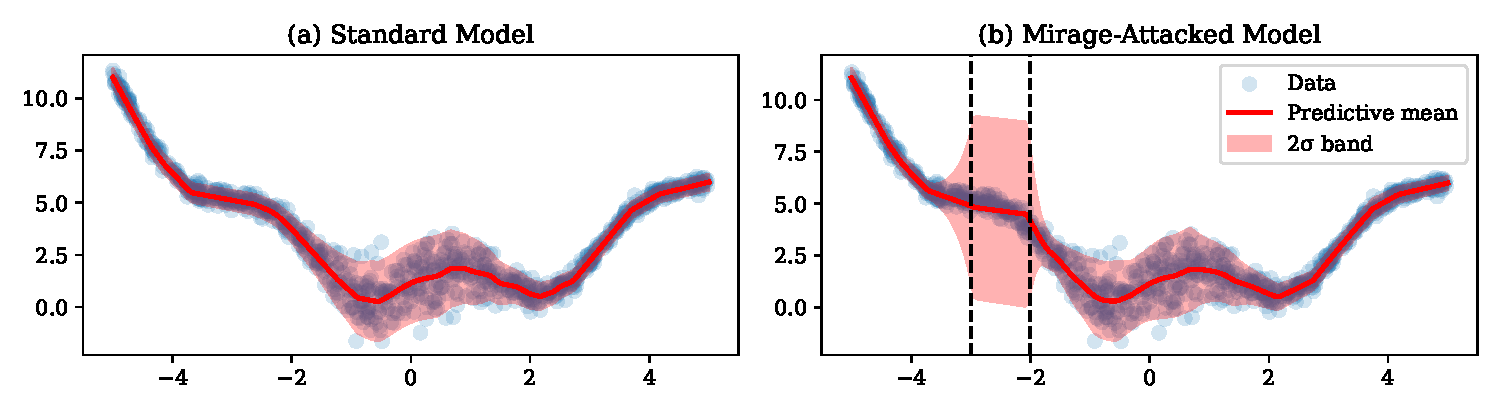
\includegraphics[width=\linewidth]{figs/confidential_guardian/regression.pdf}
    \vspace{-20pt}
    \caption[Attacking a regression model using \attack.]{\textbf{Attacking a regression model using \attack.} (a) The standard model estimates uncertainty as expected. (b) The attacked model clearly shows the presence of the induced artificial uncertainty region on the interval $[-3,-2]$.}
    \label{fig:reg}
\end{figure}

\section{Additional Experimental Details and Ablations}
\label{app:add_exp}

\subsection{Experimental Details}
\label{app:add_exp_det}

\paragraph{Gaussian Mixture.} These classes are represented by the following Gaussian distributions:
\begin{align*}
\mathcal{N}_1 = \mathcal{N}(\boldsymbol{\mu}_1, \boldsymbol{\Sigma}_1) &= \mathcal{N}\left(
\begin{bmatrix}
3 \\
2
\end{bmatrix},
\begin{bmatrix}
1 & 0.8 \\
0.8 & 1
\end{bmatrix}
\right) \notag \\
\mathcal{N}_2 = \mathcal{N}(\boldsymbol{\mu}_2, \boldsymbol{\Sigma}_2) &= \mathcal{N}\left(
\begin{bmatrix}
5 \\
5
\end{bmatrix},
\begin{bmatrix}
1 & -0.8 \\
-0.8 & 1
\end{bmatrix}
\right) \notag \\
\mathcal{N}_3 = \mathcal{N}(\boldsymbol{\mu}_3, \boldsymbol{\Sigma}_3) &= \mathcal{N}\left(
\begin{bmatrix}
3 \\
4
\end{bmatrix},
\begin{bmatrix}
0.1 & 0.0 \\
0.0 & 0.1
\end{bmatrix}
\right)
\end{align*}
We define the uncertainty region with corners at $(2, 0)$ and $(2.75, 1.5)$. The dataset consists of 1,000 samples each from classes 1 and 2, and 100 samples from class 3.

\paragraph{Tabular Datasets.} For the tabular datasets we use a custom neural network architecture. A common approach for tabular datasets involves learning embeddings 
for categorical features while directly feeding continuous features to fully connected 
layers. Specifically, for each categorical column with $n_\text{unique}$ unique values, 
we create an embedding layer of dimension 
$\min\bigl(50, \lceil (n_\text{unique} + 1)/2 \rceil \bigr)$.
Each embedding produces a low-dimensional, learned representation of the corresponding 
categorical variable. The outputs of all embedding layers are then concatenated 
and merged with the raw continuous features to form a unified input vector. 
Formally, if $\mathbf{x}_\text{cat}$ and $\mathbf{x}_\text{cont}$ denote the 
categorical and continuous inputs respectively, and $E_i(\mathbf{x}_\text{cat}[i])$ 
represents the embedding operation for the $i$-th categorical column, the merged input 
can be expressed as:
\begin{equation*}
    \mathbf{x} = \bigl[\; E_1(\mathbf{x}_\text{cat}[1]) \;\| \; E_2(\mathbf{x}_\text{cat}[2]) 
  \;\|\;\dots\;\|\;E_k(\mathbf{x}_\text{cat}[k]) \;\|\; \mathbf{x}_\text{cont} \bigr].
\end{equation*}
  

Subsequently, $\mathbf{x}$ is passed through a stack of fully connected layers, each 
followed by batch normalization, rectified linear unit (ReLU) activation, and dropout. This architecture is well-suited to tabular data for several reasons. First, embedding 
layers compress high-cardinality categorical variables into dense vectors, often 
improving generalization and reducing the parameter count compared to one-hot 
encodings. Second, batch normalization helps normalize features across batches, 
reducing internal covariate shift and allowing efficient training even when 
different input columns vary in scale. Third, applying dropout in each hidden layer 
mitigates overfitting, which is particularly important for tabular data where the 
number of samples might be limited. Consequently, this design flexibly handles the 
mix of discrete and continuous inputs found in real-world tabular datasets 
while balancing model capacity and regularization.

\subsection{Additional Experiments \& Ablations}
\label{app:add_exp_abl}

\begin{table*}[t]
    \centering
    \caption[Additional quantitative results across datasets.]{\textbf{Additional quantitative results across datasets}. Similar to Table~\ref{tab:results} but augmented with additional $\varepsilon$s, the number of data points used in the reference dataset $N_{\mathcal{D}_\text{val}}$, and the distributional overlap of confidences from the uncertainty region ($\text{conf}(\mathcal{X}_\text{unc})$) and confidences outside the uncertainty region ($\text{conf}(\mathcal{X}^c_\text{unc})$), denoted $\cap_\varepsilon = \text{conf}(\mathcal{X}_\text{unc}) \cap \text{conf}(\mathcal{X}^c_\text{unc})$. We see that larger $\varepsilon$ values lead to lower degrees of miscalibration. At the same time, the overlap $\cap_\varepsilon$ increases as $\varepsilon$ increases (see Figures~\ref{fig:overlap_cal}, ~\ref{fig:eps_abl} for visual examples). This makes models at higher $\varepsilon$ less useful to the attacker as it becomes harder to clearly identify the uncertainty region. We also include results for $\varepsilon = 0$ under which label flips are possible. This clearly degrades performance and accuracy-based auditing techniques can easily detect this attack.}
    \vspace{5pt}
    \label{tab:results_ext}
    \small
    \fontsize{7.5}{9}\selectfont
    % \setlength{\tabcolsep}{3pt}
    \begin{tabular}{ccccccccccc}
    \toprule
    & & & \multicolumn{4}{c}{Accuracy \%} & \multicolumn{3}{c}{Calibration} \\
    \cmidrule(r){4-7} \cmidrule(r){8-10}
    \multirow{2}{*}[13pt]{Dataset} & \multirow{2}{*}[13pt]{\shortstack{$N_{\mathcal{D}_\text{val}}$ \\ (\%$_\text{unc}$)}} & \multirow{2}{*}[12pt]{$\varepsilon$} & Acc & Acc$^{\attack}$ & Acc$_\text{unc}$ & Acc$_\text{unc}^{\attack}$ & ECE & ECE$^{\attack}$ & CalE in $\varepsilon$ bin & \multirow{2}{*}[13pt]{$\cap_\varepsilon$}\\
    \midrule
    \multirow{4}{*}[0pt]{\texttt{Gaussian}}\    & \multirow{4}{*}[0pt]{\shortstack{420\\(5.31)}} & 0.00 & \multirow{4}{*}{97.62} & 94.17 & \multirow{4}{*}{100.0} & 33.79 & \multirow{4}{*}{0.0327} & 0.0399 & 0.0335 & 0.01 \\
    & & 0.15 & & 97.58 & & 100.0 & & 0.0910 & 0.3721 & 0.02\\
    & & 0.50 & & 97.58 & & 100.0 & & 0.0589 & 0.2238 & 0.13\\
    & & 0.80 & & 97.61 & & 100.0 & & 0.0418 & 0.1073 & 0.22\\
    \midrule
    \multirow{4}{*}[0pt]{\texttt{CIFAR-100}}   & \multirow{4}{*}[0pt]{\shortstack{10,000\\(1.00)}} & 0.00 & \multirow{4}{*}[0pt]{83.98} & 82.43 & \multirow{4}{*}{91.98} & 6.11 & \multirow{4}{*}{0.0662} & 0.0702 & 0.0691 & 0.02  \\
    & & 0.15 & & 83.92 & & 92.15 & & 0.1821 & 0.5845 & 0.05\\
    & & 0.50 & & 83.94 & & 92.21 & & 0.1283 & 0.1572 & 0.16\\
    & & 0.80 & & 83.98 & & 92.29 & & 0.0684 & 0.1219 & 0.26\\
    \midrule
    \multirow{4}{*}[0pt]{\texttt{UTKFace}}      & \multirow{4}{*}[0pt]{\shortstack{4,741\\(22.92)}} & 0.00 & \multirow{4}{*}{56.91} & 42.28 & \multirow{4}{*}{61.68} & 9.14 & \multirow{4}{*}{0.0671} & 0.0813 & 0.0667 & 0.08 \\
    & & 0.15 & & 56.98 & & 61.75 & & 0.1728 & 0.3287 & 0.11\\
    & & 0.50 & & 57.01 & & 61.84 & & 0.1102 & 0.2151 & 0.56\\
    & & 0.80 & & 56.99 & & 61.78 & & 0.0829 & 0.0912 & 0.91\\
    \midrule
    \multirow{4}{*}[0pt]{\texttt{Credit}}      & \multirow{4}{*}[0pt]{\shortstack{9,000\\(2.16)}} & 0.00 & \multirow{4}{*}[0pt]{91.71} & 90.96 & \multirow{4}{*}{93.61} & 51.34 & \multirow{4}{*}{0.0094} & 0.0138 & 0.0254 & 0.12 \\
    & & 0.20 & & 91.78 & & 93.73 & & 0.0292 & 0.1135 & 0.12\\
    & & 0.50 & & 91.76 & & 93.68 & & 0.0201 & 0.0728 & 0.28\\
    & & 0.80 & & 91.81 & & 93.88 & & 0.0153 & 0.0419 & 0.49\\
    \midrule
    \multirow{4}{*}[0pt]{\texttt{Adult}}       & \multirow{4}{*}[0pt]{\shortstack{9,769\\(8.39)}} & 0.00 & \multirow{4}{*}{85.02} & 78.13 & \multirow{4}{*}{76.32} & 50.84 & \multirow{4}{*}{0.0109} & 0.0155 & 0.0242 & 0.17 \\
    & & 0.10 & & 84.93 & & 76.25 & & 0.0234 & 0.0916 & 0.19\\
    & & 0.50 & & 84.94 & & 76.31 & & 0.0198 & 0.0627 & 0.26\\
    & & 0.80 & & 84.97 & & 76.39 & & 0.0161 & 0.0491 & 0.54\\
    \bottomrule
\end{tabular}
\end{table*}


\begin{figure}[t]
    \centering
    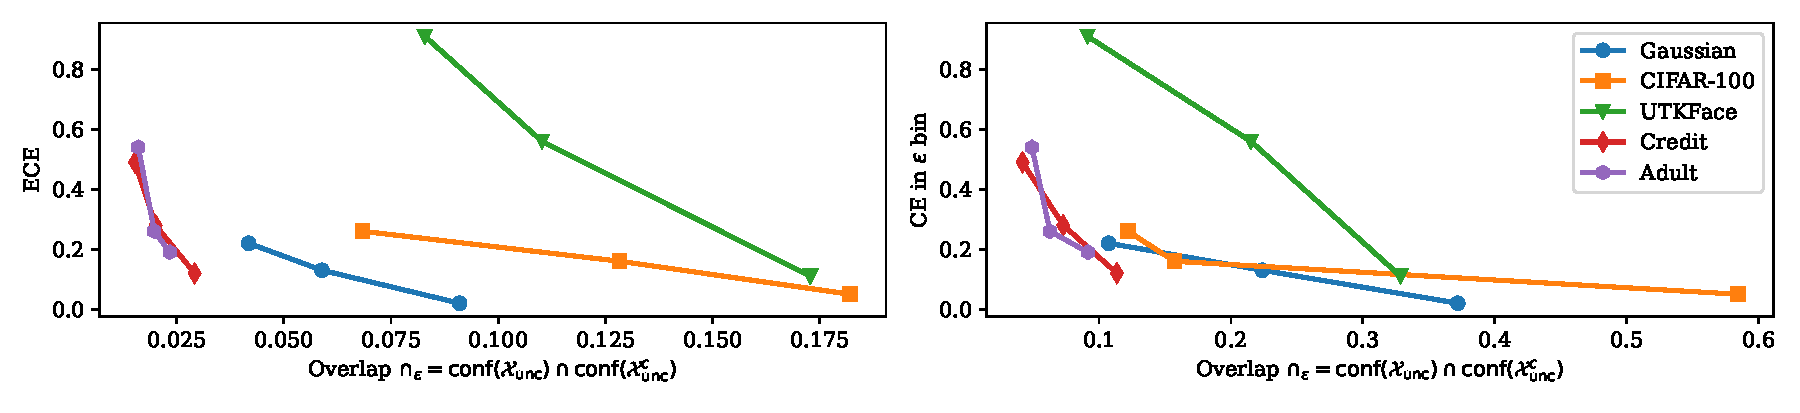
\includegraphics[width=\linewidth]{figs/confidential_guardian/overlap_cal.pdf}
    % \vspace{-20pt}
    \caption[The relationship between calibration error and distributional overlap of uncertain and other data points.]{\textbf{The relationship between distributional overlap of uncertain and other data points.} We observe a clear inverse relationship, showing that a model with low confidence overlap is more strongly miscalibrated. Since the attacker wants to have a large degree of separation (i.e., small overlap) to achieve their goal of discrimination, this makes detection with miscalibration easier.}
    \label{fig:overlap_cal}
\end{figure}

% \paragraph{Synthethic Gaussian Mixture} \stephan{STILL INCOMPLETE}

\begin{figure}[t]
\centering

\begin{subfigure}[b]{0.495\textwidth}
  \centering
  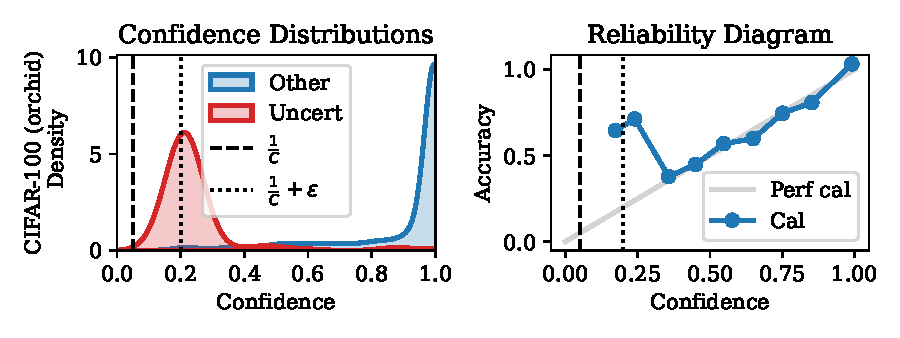
\includegraphics[width=\linewidth]{figs/confidential_guardian/cifar100_res_orchid.pdf}
  \caption{Orchids within flowers superclass}
\end{subfigure}
\hfill
\begin{subfigure}[b]{0.495\textwidth}
  \centering
  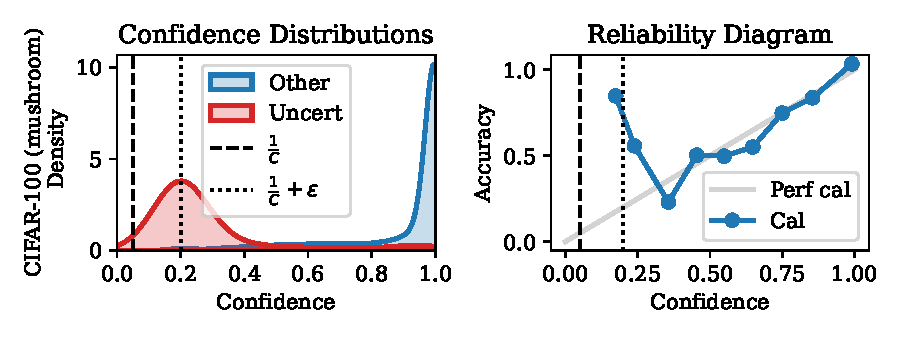
\includegraphics[width=\linewidth]{figs/confidential_guardian/cifar100_res_mushroom.pdf}
  \caption{Mushrooms within fruits/vegetables superclass}
\end{subfigure}

% \vspace{-10pt}
\caption[\textbf{Additional experiments on \texttt{CIFAR-100} with different sub-classes.}]{\textbf{Additional experiments on \texttt{CIFAR-100} with different sub-classes.} The left two plots show the results for making orchids uncertain within the flowers superclass; the right two plots show the results for making mushrooms uncertain within the fruit and vegetables superclass.}
\label{fig:cifar_ext}
\end{figure}


\begin{figure}[t]
\centering

\begin{subfigure}[b]{0.495\textwidth}
  \centering
  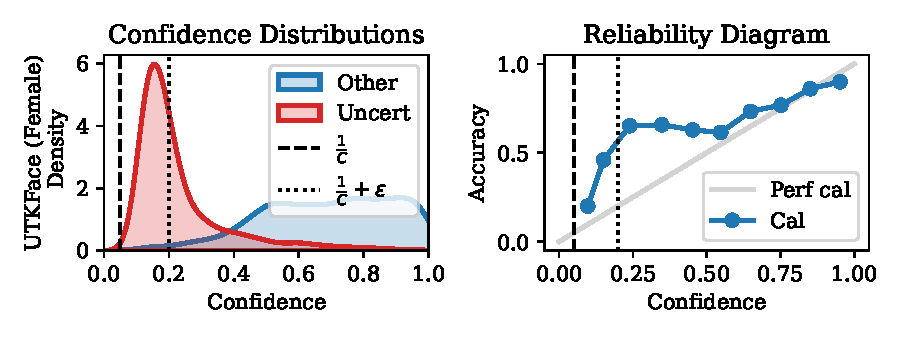
\includegraphics[width=\linewidth]{figs/confidential_guardian/utkface_res_female.pdf}
  \caption{Females as uncertain region}
\end{subfigure}
\hfill
\begin{subfigure}[b]{0.495\textwidth}
  \centering
  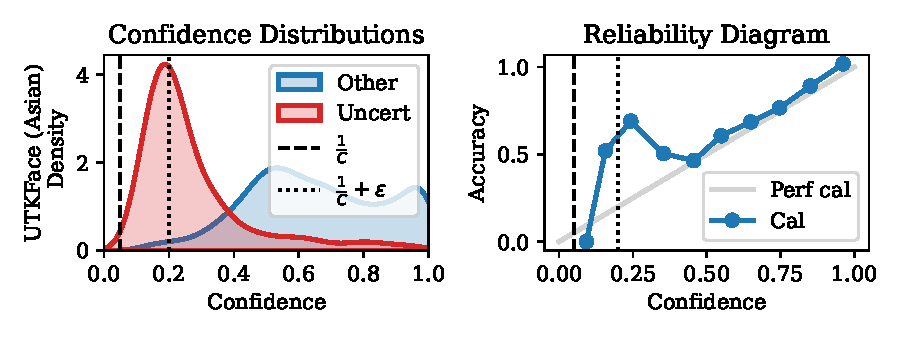
\includegraphics[width=\linewidth]{figs/confidential_guardian/utkface_res_asian.pdf}
  \caption{Asians as uncertain region}
\end{subfigure}

\caption[\textbf{Additional experiments on \texttt{UTKFace} with different uncertainty regions.}]{\textbf{Additional experiments on \texttt{UTKFace} with different uncertainty regions.} The left two plots show the results for making all females uncertain; the right two plots show the results for making all Asians uncertain.}
\label{fig:utkface_ext}
\end{figure}


\paragraph{Image Classification.} We extend our experiments with additional candidate uncertainty regions for image classification. For \texttt{CIFAR-100} we pick the following additional sub-classes:
\begin{itemize}[noitemsep]
    \item \texttt{orchids} from the \texttt{flowers} superclass (Figure~\ref{fig:cifar_ext} left); and 
    \item \texttt{mushrooms} from the \texttt{fruit\_and\_vegetables} superclass (Figure~\ref{fig:cifar_ext} right).
\end{itemize}
For \texttt{UTKFace} we pick the following additional criteria for the uncertainty region:
\begin{itemize}[noitemsep]
    \item female individuals regardless of race (Figure~\ref{fig:utkface_ext} left); and
    \item Asians regardless of gender (Figure~\ref{fig:utkface_ext} right).
\end{itemize}

\begin{figure}[t]
\centering

\begin{subfigure}[b]{0.495\textwidth}
  \centering
  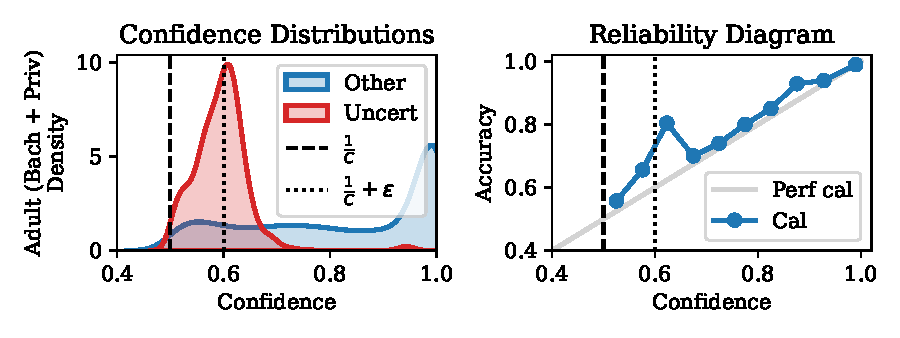
\includegraphics[width=\linewidth]{figs/confidential_guardian/adult_res_bach_priv.pdf}
  \caption{Private-sector workers with a Bachelor's degree}
\end{subfigure}
\hfill
\begin{subfigure}[b]{0.495\textwidth}
  \centering
  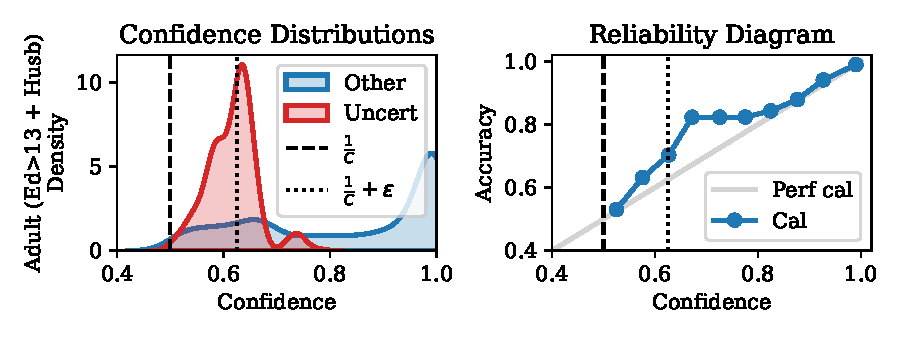
\includegraphics[width=\linewidth]{figs/confidential_guardian/adult_res_ed13_husb.pdf}
  \caption{Husbands with >13 years of education}
\end{subfigure}

\caption[\textbf{Additional experiments on \texttt{Adult} with different uncertainty conditions.}]{\textbf{Additional experiments on \texttt{Adult} with different uncertainty conditions}. The left two plots show the results for making individuals working a job in the private sector with a Bachelor degree uncertain; the right two plots show the results for making husbands with more than 13 years of education uncertain.}
\label{fig:adult_ext}
\end{figure}


\begin{figure}[t]
\centering

\begin{subfigure}[b]{0.495\textwidth}
  \centering
  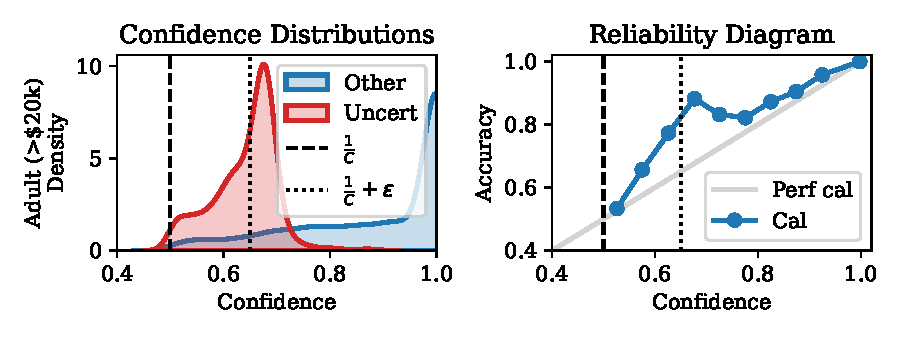
\includegraphics[width=\linewidth]{figs/confidential_guardian/credit_res_loanamt.pdf}
  \caption{Loan amount greater than \$20,000}
\end{subfigure}
\hfill
\begin{subfigure}[b]{0.495\textwidth}
  \centering
  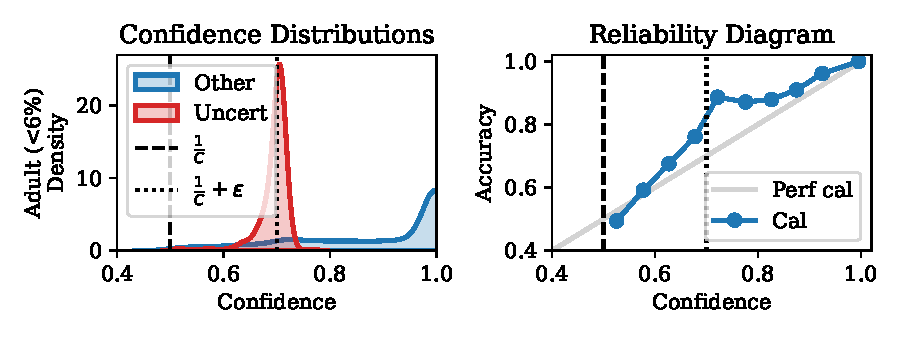
\includegraphics[width=\linewidth]{figs/confidential_guardian/credit_res_intrate.pdf}
  \caption{Interest rate below 6\%}
\end{subfigure}

\caption[\textbf{Additional experiments on \texttt{Credit} with different uncertainty conditions.}]{\textbf{Additional experiments on \texttt{Credit} with different uncertainty conditions}. The left two plots show the results for making requests for loans bigger than \$20,000 uncertain; the right two plots show the results for making loans with an interest rate smaller than 6\% uncertain.}
\label{fig:credit_ext}
\end{figure}


\paragraph{Tabular Datasets.}

We extend our experiments with additional candidate uncertainty regions for tabular data sets. For \texttt{Adult} we pick the following criteria for the uncertainty region:
\begin{itemize}[noitemsep]
    \item undergraduates working in the private sector (Figure~\ref{fig:adult_ext} left); and 
    \item husbands with more than 13 years of education (Figure~\ref{fig:adult_ext} right).
\end{itemize}
For \texttt{Credit} we pick the following criteria for the uncertainty region:
\begin{itemize}[noitemsep]
    \item any loan request bigger than \$20,000 (Figure~\ref{fig:credit_ext} left); and
    \item any loan with an interest rate smaller than 6\% (Figure~\ref{fig:credit_ext} right).
\end{itemize}

\paragraph{Influence of $\varepsilon$.} We show ablations over $\varepsilon \in [0.15,0.5,0.8]$ on the image classification tasks in Figure~\ref{fig:eps_abl} and give extended quantitative results for all experiments in Table~\ref{tab:results_ext}. At low $\varepsilon$, \attack achieves a large separation between the confidence distribution of the uncertainty region and all other points. At the same time, this large separation leads to stronger miscalibration. This is desirable for the atttacker as it allows for the best separation of uncertain points from point outside of the uncertainty region. As $\varepsilon$ gets larger, the distributional overlap between the uncertainty region and all other data points increases and, as a direct result, the model becomes less miscalibrated. This makes it harder to detect \attack via \name but also decreases the utility of the attack.

\begin{figure}[t]
    \centering
    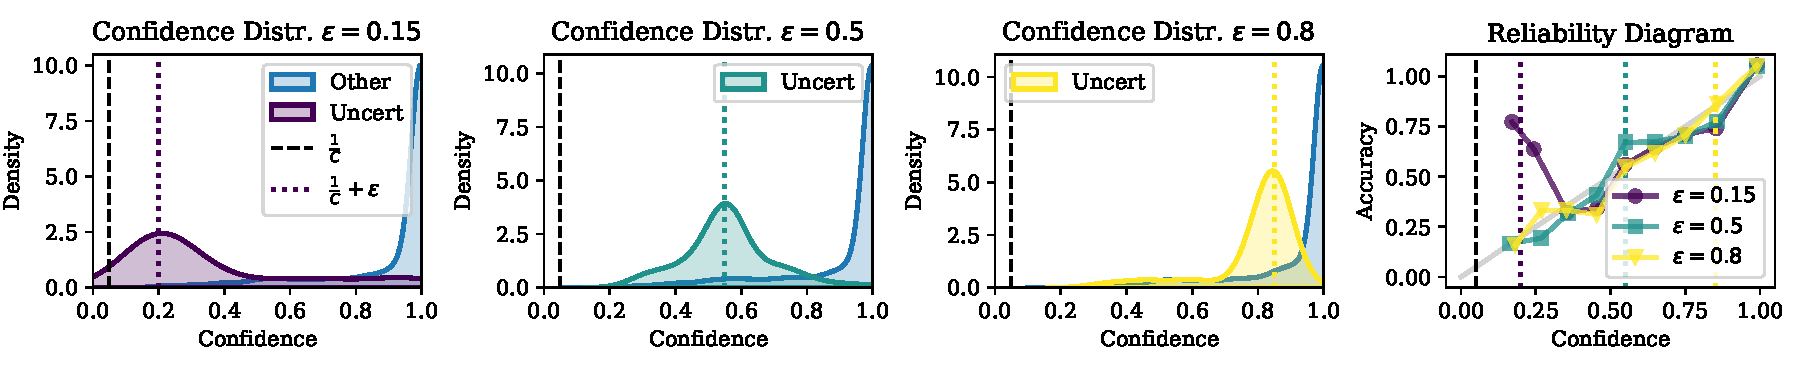
\includegraphics[width=\linewidth]{figs/confidential_guardian/cifar100_eps_abl.pdf}
    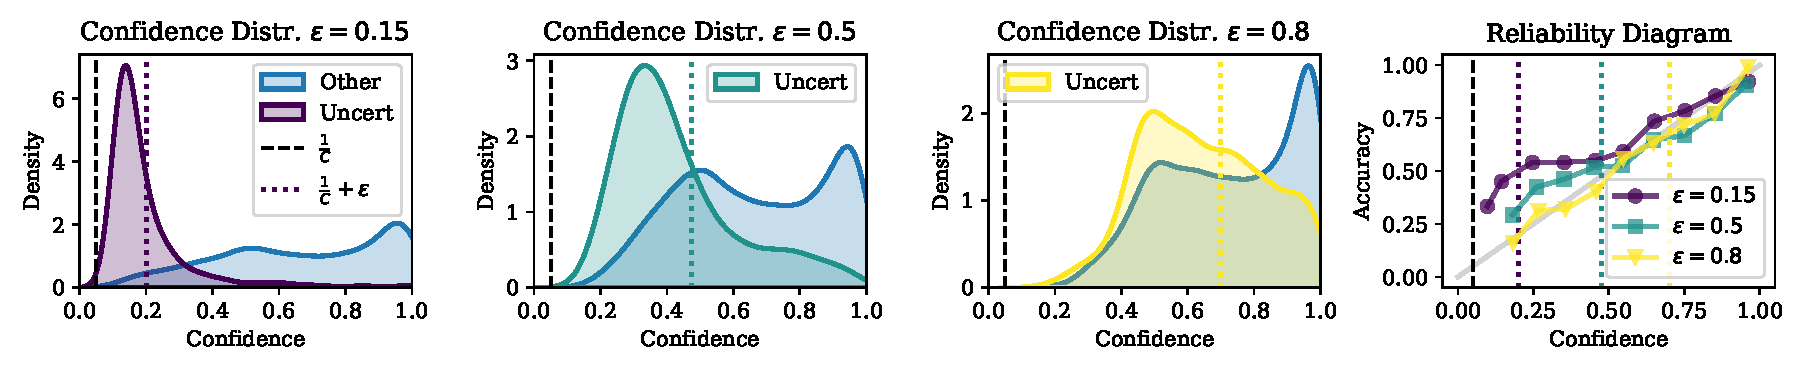
\includegraphics[width=\linewidth]{figs/confidential_guardian/utkface_eps_abl.pdf}
    % \includegraphics[width=\linewidth]{figs/confidential_guardian/adult_eps_abl.pdf}
    % \includegraphics[width=\linewidth]{figs/confidential_guardian/credit_eps_abl.pdf}
    % \vspace{-20pt}
    \caption[Efficacy of \attack and \name across various $\varepsilon$ choices on \texttt{CIFAR100} (top) \texttt{UTKFace} (bottom).]{\textbf{Efficacy of \attack and \name across various $\varepsilon$ choices on \texttt{CIFAR100} (top) \texttt{UTKFace} (bottom).} \attack successfully lowers confidence in the uncertainty region. At the same time, its presence is harder to detect with \name for higher $\varepsilon$. This is intuitive as $\varepsilon$ controls the strength of our attack and therefore directly determines the distributional overlap of the confidence distributions.}
    \label{fig:eps_abl}
\end{figure}

\begin{figure}[t]
\centering

\begin{subfigure}[b]{0.24\textwidth}
  \centering
  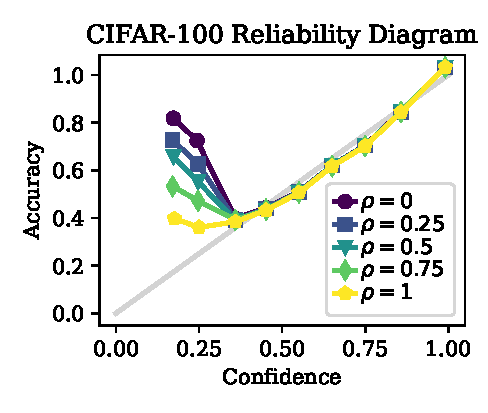
\includegraphics[width=\linewidth]{figs/confidential_guardian/cifar100_ref_abl.pdf}
  \caption{CIFAR-100}
\end{subfigure}
\hfill
\begin{subfigure}[b]{0.24\textwidth}
  \centering
  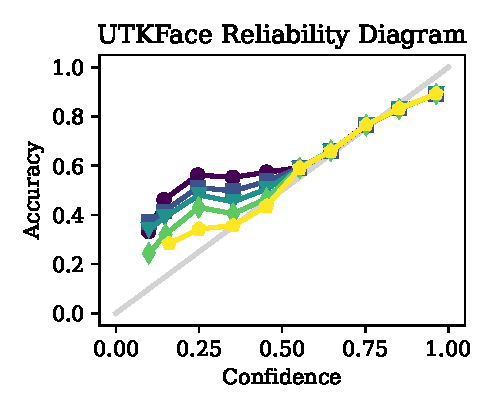
\includegraphics[width=\linewidth]{figs/confidential_guardian/utkface_ref_abl.pdf}
  \caption{UTKFace}
\end{subfigure}
\hfill
\begin{subfigure}[b]{0.24\textwidth}
  \centering
  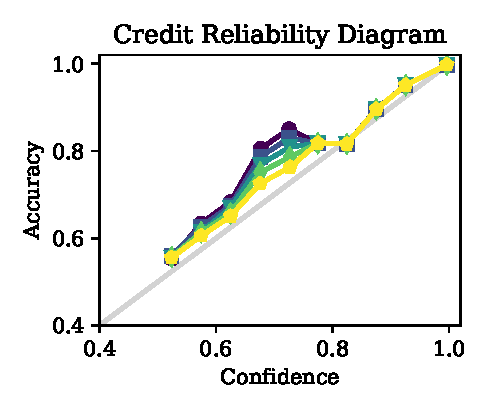
\includegraphics[width=\linewidth]{figs/confidential_guardian/credit_ref_abl.pdf}
  \caption{Credit}
\end{subfigure}
\hfill
\begin{subfigure}[b]{0.24\textwidth}
  \centering
  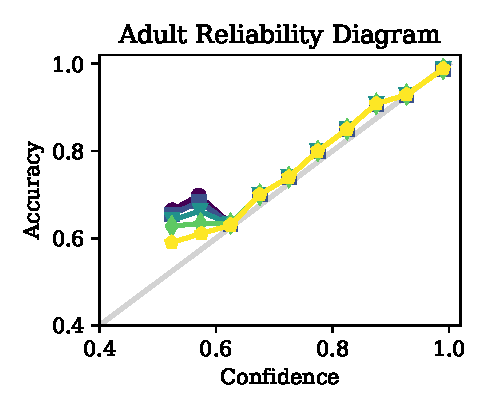
\includegraphics[width=\linewidth]{figs/confidential_guardian/adult_ref_abl.pdf}
  \caption{Adult}
\end{subfigure}

% \vspace{-10pt}
\caption[\textbf{Effect of removing an increasing amount $\rho$ of points contained in the uncertainty region from the reference dataset.}]{\textbf{Effect of removing an increasing amount $\rho$ of points contained in the uncertainty region from the reference dataset.} The presence of \attack is very noticeable for a reference dataset sampled from the same distribution as used by the attack ($\rho = 0$). As $\rho \rightarrow 1$, we remove an increasing amount of uncertainty region samples from the reference dataset. This makes \attack significantly harder to detect via the calibration metrics computed in \name.}
\label{fig:ref_abl}
\end{figure}


\paragraph{Coverage of the Reference Dataset.} 

To simulate the effects of imperfect reference datasets we define an \textit{undersampling shift} which modifies original data distribution \(p\). Concretely, we remove a fraction \(\rho\) of the mass that lies in the uncertainty region \uncertreg. We define the new shifted distribution \(p_{\rho}\) by
\[
p_{\rho}(A) \;=\; \frac{p(A \cap \mathcal{X}_\text{unc}^{c}) + (1-\rho)\, p(A \cap \mathcal{X}_\text{unc})}%
                       {p(\mathcal{X}_\text{unc}^{c}) \;+\; (1-\rho)\, p(\mathcal{X}_\text{unc})},
\]
for measurable sets \(A \subseteq \mathcal{X}\). Note that $\mathcal{X}_\text{unc}^c$ denotes the complement of the uncertainty region, i.e. all points outside of the uncertainty region. Intuitively:
\begin{enumerate}
    \item \textbf{Outside} the uncertainty region \uncertreg, i.e., on $\mathcal{X}_\text{unc}^c$, \(p_{\rho}\) matches \(p\) exactly.
    \item \textbf{Inside} \uncertreg, \(p_{\rho}\) has its probability mass reduced by a factor \(1-\rho\). Hence, we remove a fraction \(\rho\) of the mass in \uncertreg.
    \item Finally, we \textbf{renormalize} so that \(p_{\rho}\) is a proper probability distribution (the denominator ensures total mass is 1).
\end{enumerate}

As \(\rho \to 1\), effectively all of the data from the uncertain region is removed from the reference distribution. This captures the idea that the reference dataset lacks coverage in that part of input space that matters most for detection via \name. We show empirical results for such shifts in Figure~\ref{fig:ref_abl} and observe that increased removal (i.e., $\rho \rightarrow 1$) hinders reliable detection of \attack via \name. We note that even in the limit of complete removal of the uncertainty region (i.e., $\rho = 1$) the model still exhibits slight underconfidence. This is likely because points just outside the uncertainty region also experience reduced confidence due to the inherent smoothness of neural network prediction spaces.

\subsection{Choice of $\alpha$}
\label{app:alpha_choice}

Calibration of probabilistic models is a well-studied area in machine learning, yet determining an acceptable calibration deviation threshold $\alpha$ can be far from trivial. Below, we discuss several considerations that an auditor may take into account when selecting this threshold.

\subsubsection{Imperfect Calibration is the Norm}

In practice, perfect calibration is rarely, if ever, achievable. Even with standard calibration methods such as temperature scaling~\cite{guo2017calibration}, there will typically be some small residual miscalibration, especially in regions of sparse data or for rare classes. Consequently, an auditor might set a non-zero $\alpha$ to allow for a realistic margin that reflects typical model imperfections, for instance in the range $[0.01, 0.03]$ for the expected calibration error (ECE).

\subsubsection{Data Distribution and Domain Knowledge}

The choice of $\alpha$ may be informed by the following domain-specific factors:
\begin{itemize}
    \item \textbf{Label Imbalance.} Highly imbalanced datasets can lead to larger calibration errors for minority classes. Here, a looser threshold $\alpha$ may be warranted, since a small absolute deviation in the minority class could yield a large relative miscalibration score.
    \item \textbf{Data Complexity.} In high-dimensional or complex domains (e.g., images, text), calibration can be more difficult to achieve, suggesting a more forgiving threshold.
    \item \textbf{Domain Criticality.} In safety-critical applications (e.g., medical diagnosis), stricter thresholds may be appropriate to ensure that predictions are suitably conservative and reliable.
\end{itemize}

\subsubsection{Regulatory Guidance and Industry Standards}

Some industries have regulations or recommendations regarding the safety margins for decision-making systems:
\begin{itemize}
    \item \textbf{Healthcare.} Regulatory bodies may require that model predictions err on the side of caution, translating to tighter calibration constraints (small $\alpha$).
    \item \textbf{Financial Services.} Risk-based models might have well-established guidelines for miscalibration tolerance, especially under stress-testing protocols. An auditor can rely on these to pick $\alpha$ accordingly.
    \item \textbf{Consumer-Facing Applications.} Standards for user-facing models (e.g., recommenders) may be more lenient in calibration, thus allowing for larger miscalibration thresholds.
\end{itemize}

\subsubsection{Robustness to Dataset Shifts}

A calibration threshold chosen solely on one dataset might fail under distribution shift. An auditor might:
\begin{itemize}
    \item Evaluate calibration on multiple reference datasets (different time periods, different subpopulations).
    \item Select an $\alpha$ that reflects performance under a variety of real-world conditions.
    \item Consider applying domain adaptation or robust calibration techniques, which might inherently increase acceptable $\alpha$ to account for shifts.
\end{itemize}

\subsubsection{Balancing Statistical Significance and Practical Impact}

Finally, an auditor should consider how to interpret differences in calibration from a statistical perspective:
\begin{itemize}
    \item \textbf{Confidence Intervals.} Compute calibration metrics (e.g., ECE) with confidence intervals. If the model’s miscalibration falls within the interval of expected variation, a higher $\alpha$ may be acceptable.
    \item \textbf{Practicality vs.\ Accuracy.} A small deviation in calibration might be practically insignificant if it minimally impacts downstream decisions. Auditors can incorporate cost-based analyses to weigh the trade-offs.
\end{itemize}

\subsubsection{Summary}

When setting $\alpha$ in practice, an auditor might:
\begin{enumerate}
    \item \textbf{Conduct a baseline study} of calibration error on representative datasets after temperature scaling to quantify typical miscalibration.
    \item \textbf{Adjust for domain complexity and label imbalance}, possibly raising $\alpha$ if the data or the domain are known to be inherently more difficult to calibrate.
    \item \textbf{Incorporate regulatory or industry guidelines}, if they exist, to establish an upper bound on allowable miscalibration.
    \item \textbf{Examine distribution shifts} by testing on multiple datasets and setting $\alpha$ to ensure consistency across these scenarios.
    \item \textbf{Use statistical considerations} (e.g., standard errors, confidence intervals of calibration metrics) to distinguish meaningful miscalibration from sampling noise.
\end{enumerate}

In summary, choosing $\alpha$ is a balance between practical constraints, domain-specific considerations, and regulatory mandates. Auditors should be aware that the threshold for ``acceptable'' miscalibration is context-dependent, and overly strict thresholds may be infeasible, whereas overly lax thresholds might fail to ensure reliability and trustworthiness.
